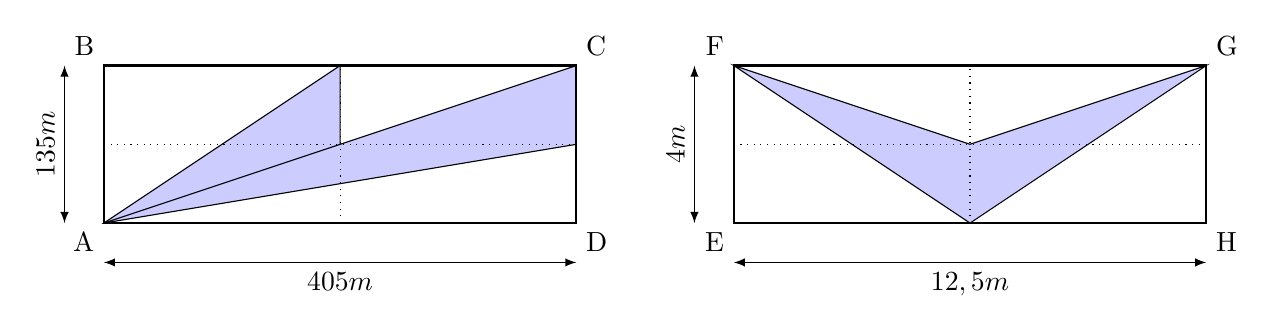
\begin{tikzpicture}
        \node[below left] at (0,0) {$\mathrm{A}$} ;
        \node[above left] at (0,2) {$\mathrm{B}$} ;
        \node[above right] at (6,2) {$\mathrm{C}$} ;
        \node[below right] at (6,0) {$\mathrm{D}$} ;
        \draw[fill=blue!20, thin] (0,0) -- (6,1) -- (6,2) -- (3,1) -- (3,2) -- cycle ;
        \draw[thick] (0,0) rectangle (6,2) ;
        \draw[dotted] (3,0) -- (3,2) ;
        \draw[dotted] (0,1) -- (6,1) ;
        \draw[thin] (0,0) -- (3,1) ;
        \draw[<->, >=latex] (0,-0.5) --node[midway, below]{$405\un{m}$} (6,-0.5) ;
        \draw[<->, >=latex] (-0.5,0) --node[midway, above, sloped]{$135\un{m}$} (-0.5,2) ;

        \begin{scope}[xshift=8cm]
        \node[below left] at (0,0) {$\mathrm{E}$} ;
        \node[above left] at (0,2) {$\mathrm{F}$} ;
        \node[above right] at (6,2) {$\mathrm{G}$} ;
        \node[below right] at (6,0) {$\mathrm{H}$} ;
        \draw[fill=blue!20, thin] (0,2) -- (3,0) -- (6,2) -- (3,1) -- cycle ;
        \draw[thick] (0,0) rectangle (6,2) ;
        \draw[dotted] (3,0) -- (3,2) ;
        \draw[dotted] (0,1) -- (6,1) ;
        \draw[<->, >=latex] (0,-0.5) --node[midway, below]{$12,5\un{m}$} (6,-0.5) ;
        \draw[<->, >=latex] (-0.5,0) --node[midway, above, sloped]{$4\un{m}$} (-0.5,2) ;
        \end{scope}
    \end{tikzpicture}